\chapter{Проектирование системы}

\section{Системная архитектура}

Кластер — это группа компьютеров, объединённых высокоскоростными каналами связи и представляющая с точки зрения пользователя единый ресурс. Это значит, что для создания кластера необходимы как минимум несколько компьютеров. В последнее время, популярными становятся услуги облачных вычислений. Потребителю таких услуг не нужно беспокоиться о настройке физических серверов, поддержке сети и прочих аппаратных проблемах. В качестве провайдера таких услуг был выбран самый популярный подобный сервис — Amazon Elastic Compute Cloud. Доступ к системе предоставляется через API. Он позволяет создавать виртуальные машины, клонировать существующие. Есть возможность выбора разных конфигураций виртуальных машин.


\begin{figure}
  \centering
  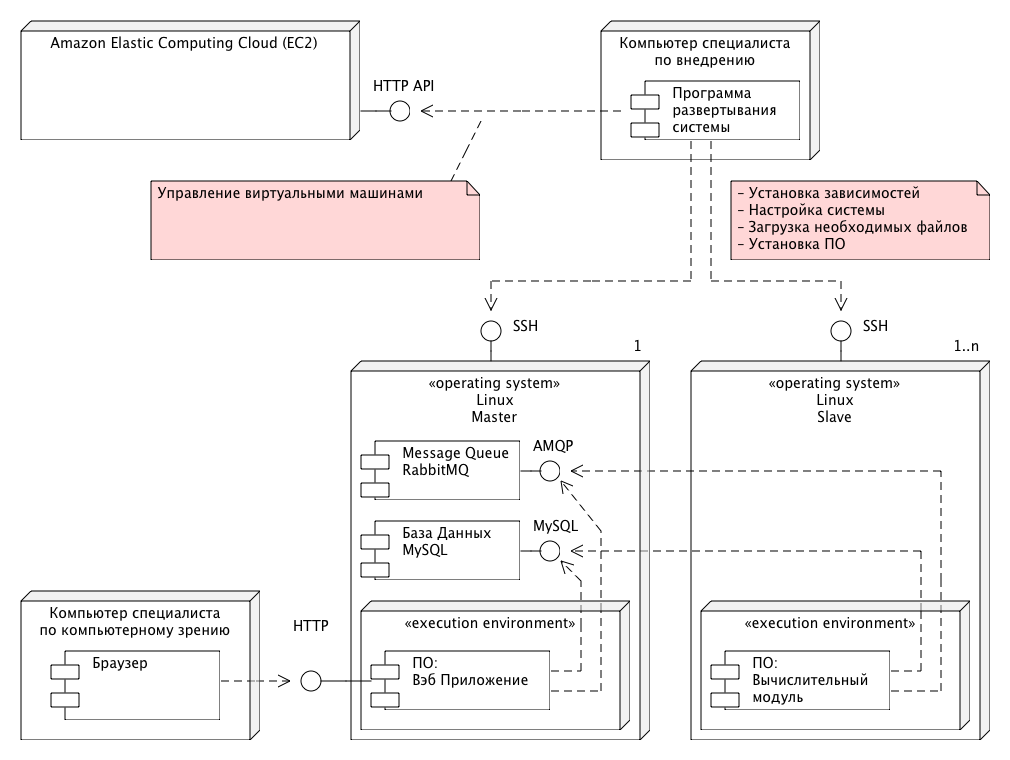
\includegraphics[width=0.8\textwidth]{assets/deploy-1.png}
  \caption{Диаграмма развертки}
  \label{fig:fig01}
\end{figure}


\section{Программная архитектура}

Классификация параллельных архитектур по Флинну определяет 4 типа параллельных систем:
\begin{enumerate}
  \item ОКОД — одиночный поток команд и одиночный поток данных;
  \item ОКМД — одиночный поток команд и множественный поток данных;
  \item МКОД — множественный поток команд и одиночный поток данных;
  \item МКМД — множественный поток команд и множественный поток данных.
\end{enumerate}

Наша система относится к 4-ому типу — вычислительная система со множественным потоком команд и множественным потоком данных.

Основными типами кластеров являются:
\begin{enumerate}
  \item Кластеры высокой доступности (High-availability clusters) — этот тип кластеров используется в случае, когда нужно обеспечить максимальную доступность сервиса. Доступность обеспечивается кол-вом серверов. Чем больше кол-во серверов, тем доступнее предоставляемый сервис.
  \item Кластеры распределения нагрузки — основная задача этого типа кластеров — повышение производительности и надежности системы путем распределении нагрузки между большим кол-вом узлов.
  \item Вычислительные кластеры — основная задача этих кластеров — быстрые вычисления. Надежность и доступность в этом случае играет маленькую роль и на первый план выходит производительность системы и удельная стоимость вычислительных ресурсов.
\end{enumerate}

По типу организации кластеров, их можно разделить на системные и программные. В первом случае объединение в один ресурс происходит на уровне ядра операционной системы. Такие системы могут перемещать процессы вместе с памятью между ядрами. Во втором случае объединение серверов в один ресурс происходит на уровне программных протоколов.

В нашем случае, разрабатываемая система является типичным примером вычислительного кластера. Мною был выбран программный подход нежели чем параллелизация на уровне ядра, по причине большей простоты и гибкости такого решения.



%Beowulf

%Диаграмма компонентов
%диаграммы UML, схемы алгоритмов.


\section{Архитектура данных}

% ERM - инфологическая
%  - диаграммы ER, инфологическая модель и даталогическая
% модель, описание основных транзакции с указанием специфичных запросов,
% хранимых процедур и триггеров.

\begin{figure}[h]
  \centering
  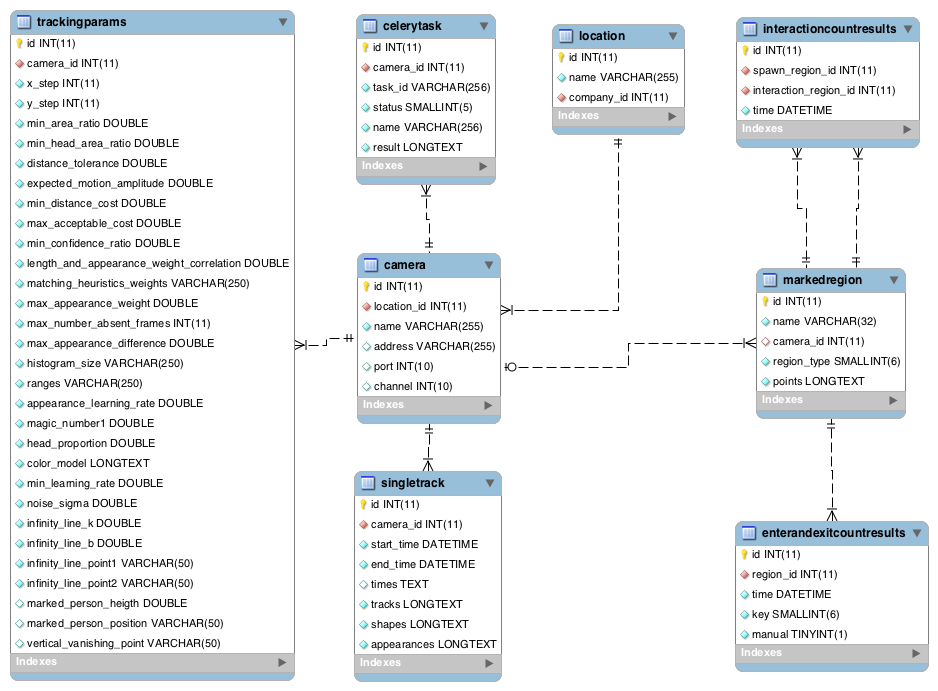
\includegraphics[width=0.8\textwidth]{assets/schema-1.png}
  \caption{Инфологическая EER модель}
  \label{fig:fig01}
\end{figure}
